\documentclass[border=10pt]{standalone}
\usepackage{tikz}
\usetikzlibrary{arrows.meta, positioning, calc}

\begin{document}

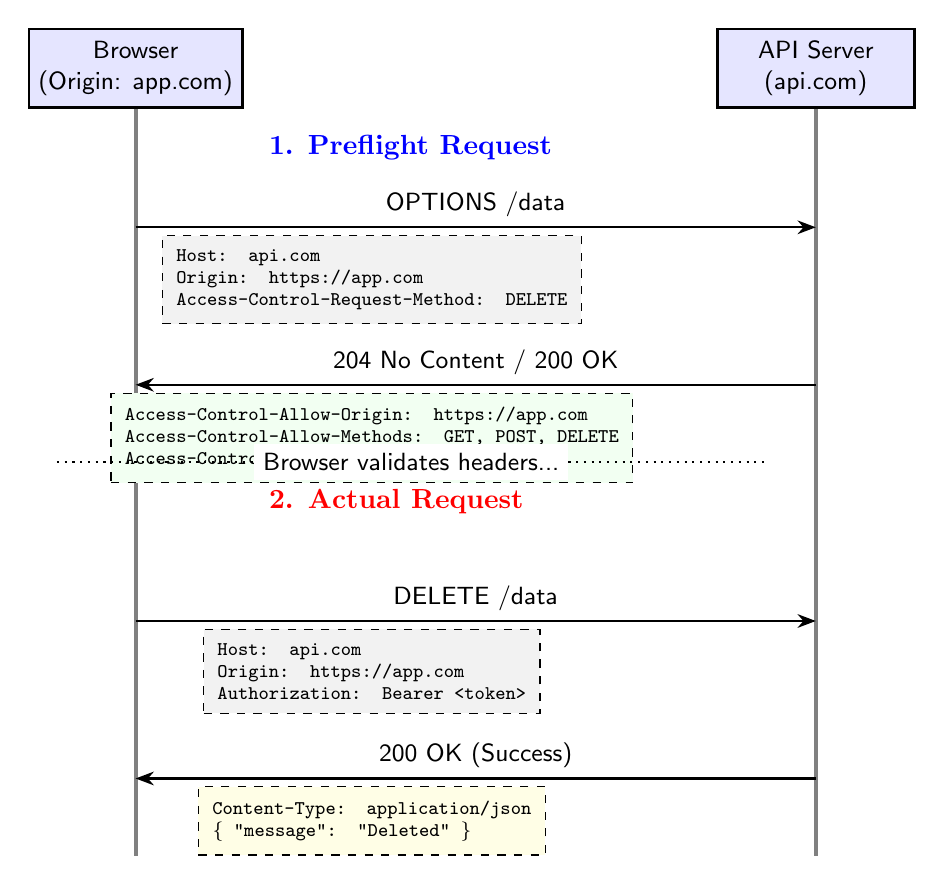
\begin{tikzpicture}[
    node distance=1.5cm,
    font=\sffamily\small,
    >=Stealth,
    box/.style={rectangle, draw, fill=blue!10, minimum width=2.5cm, minimum height=1cm, align=center, line width=1pt},
    header/.style={fill=gray!10, draw, dashed, font=\ttfamily\scriptsize, align=left, inner sep=5pt}
]

    % Lifelines
    \node[box] (browser) {Browser\\(Origin: app.com)};
    \node[box, right=6cm of browser] (server) {API Server\\(api.com)};
    
    \draw[line width=1.5pt, gray] (browser) -- ++(0,-10);
    \draw[line width=1.5pt, gray] (server) -- ++(0,-10);

    % --- PHASE 1: PREFLIGHT ---
    \node[right=0.2cm of browser, yshift=-1cm, anchor=west, font=\bfseries\color{blue}] {1. Preflight Request};
    \draw[->, thick] ($(browser.south)+(0,-1.5)$) -- ($(server.south)+(0,-1.5)$) 
        node[midway, above, align=center] {OPTIONS /data};
    
    \node[header, below=1.6cm of browser, xshift=3cm] {
        Host: api.com\\
        Origin: https://app.com\\
        Access-Control-Request-Method: DELETE
    };

    % --- PHASE 2: PREFLIGHT RESPONSE ---
    \draw[<-, thick] ($(browser.south)+(0,-3.5)$) -- ($(server.south)+(0,-3.5)$) 
        node[midway, above] {204 No Content / 200 OK};
        
    \node[header, below=3.6cm of browser, xshift=3cm, fill=green!5] {
        Access-Control-Allow-Origin: https://app.com\\
        Access-Control-Allow-Methods: GET, POST, DELETE\\
        Access-Control-Max-Age: 86400
    };

    % Separator
    \draw[dotted, thick] (-1,-5) -- (8,-5) node[midway, fill=white] {Browser validates headers...};

    % --- PHASE 3: ACTUAL REQUEST ---
    \node[right=0.2cm of browser, yshift=-5.5cm, anchor=west, font=\bfseries\color{red}] {2. Actual Request};
    \draw[->, thick] ($(browser.south)+(0,-6.5)$) -- ($(server.south)+(0,-6.5)$) 
        node[midway, above] {DELETE /data};

    \node[header, below=6.6cm of browser, xshift=3cm] {
        Host: api.com\\
        Origin: https://app.com\\
        Authorization: Bearer <token>
    };

    % --- PHASE 4: ACTUAL RESPONSE ---
    \draw[<-, thick] ($(browser.south)+(0,-8.5)$) -- ($(server.south)+(0,-8.5)$) 
        node[midway, above] {200 OK (Success)};

    \node[header, below=8.6cm of browser, xshift=3cm, fill=yellow!10] {
        Content-Type: application/json\\
        \{ "message": "Deleted" \}
    };

\end{tikzpicture}

\end{document}